	% !TeX spellcheck = en_GB
\documentclass[11pt]{beamer}
\usepackage[utf8]{inputenc}
%\usepackage[T1]{fontenc}
\usepackage[sort]{natbib}

\usetheme[compress]{Berlin} % "compress" sorgt für Horizontale Punkte in der section Kopfzeile
\usecolortheme{dolphin}

\begin{document}
	\author{Matthias Wilke \& Fabian Fey}
	\title{Project Report - TeamLab Phonetics}
%	\logo{Bilder/logo-IMS.jpg}
	\institute{Institute for Natural Language Processing}
	%\date{}
	%\subject{}
	\setbeamercovered{transparent}
	\setbeamertemplate{navigation symbols}{}
	
\begin{frame}[plain]
	\maketitle
\end{frame}


\begin{frame}
	\frametitle{Table of contents}
	\tableofcontents[hideallsubsections]
\end{frame}

\AtBeginSection[]
{
	\begin{frame}
	\frametitle{Outline}
		\tableofcontents[
		currentsection,
		currentsubsection,
		subsectionstyle=hide
		]
	\end{frame}
}

\section{New Domain}
\begin{frame}
	\frametitle{Goals}
	\begin{itemize}
		\item New domain to answer Movie related questions like: \pause
		\begin{itemize}
			\item Information about a specific actor \pause
			\item Information about a specific movie \pause
		\end{itemize}
		\item[$\Rightarrow$] Build a database and integrate it in PyDial
	\end{itemize}
\end{frame}

\section{Data Acquisition}
	\subsection{IMDB Database}
	\begin{frame}
		\begin{itemize}
			\item IMDB-Database\footnote{\url{https://www.imdb.com/interfaces/ [28.07.2018]}} \pause
			\item \textit{title.basics.tsv} \pause
			\begin{itemize}
				\item Title based database  \pause
			\end{itemize}
			\item \textit{name.basics.tsv} \pause
			\begin{itemize}
				\item Actor based database 
			\end{itemize}
		\end{itemize}
	\end{frame}

	\begin{frame}
		\frametitle{title.basics.tsv}
		\begin{figure}[ht]
			\centering
			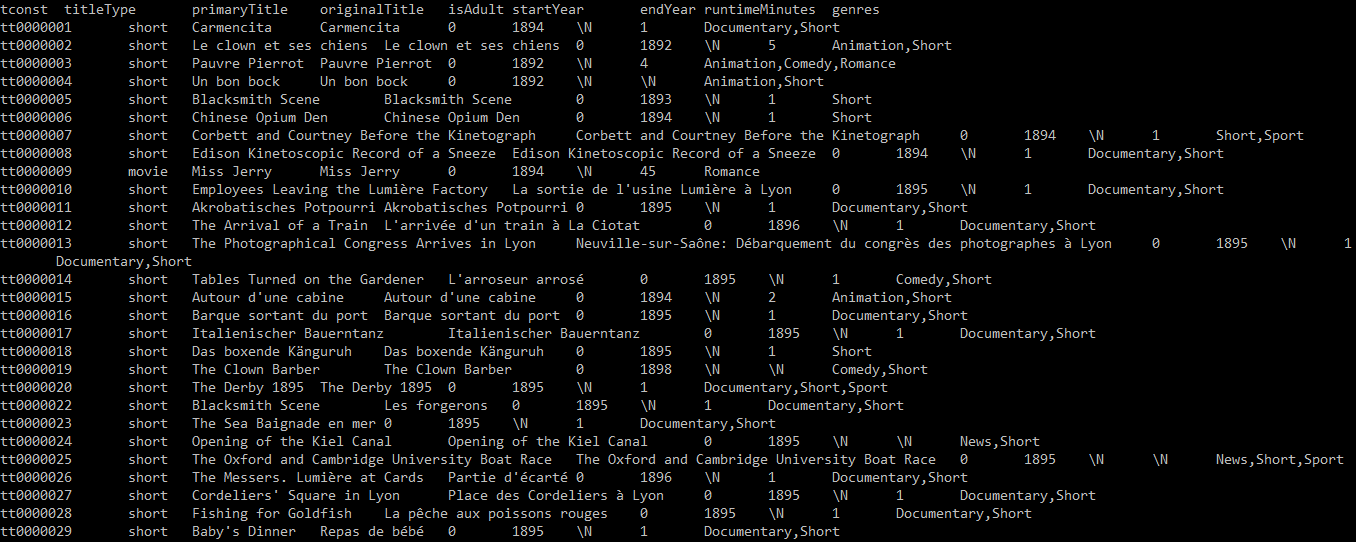
\includegraphics[width=0.8\paperwidth]{Pics/title.PNG}
			\caption{Short excerpt of the \textit{title.basics.tsv} file.}
			\label{pic:title}
		\end{figure}
	\end{frame}

	\begin{frame}
		\frametitle{names.basics.tsv}
		\begin{figure}[ht]
			\centering
			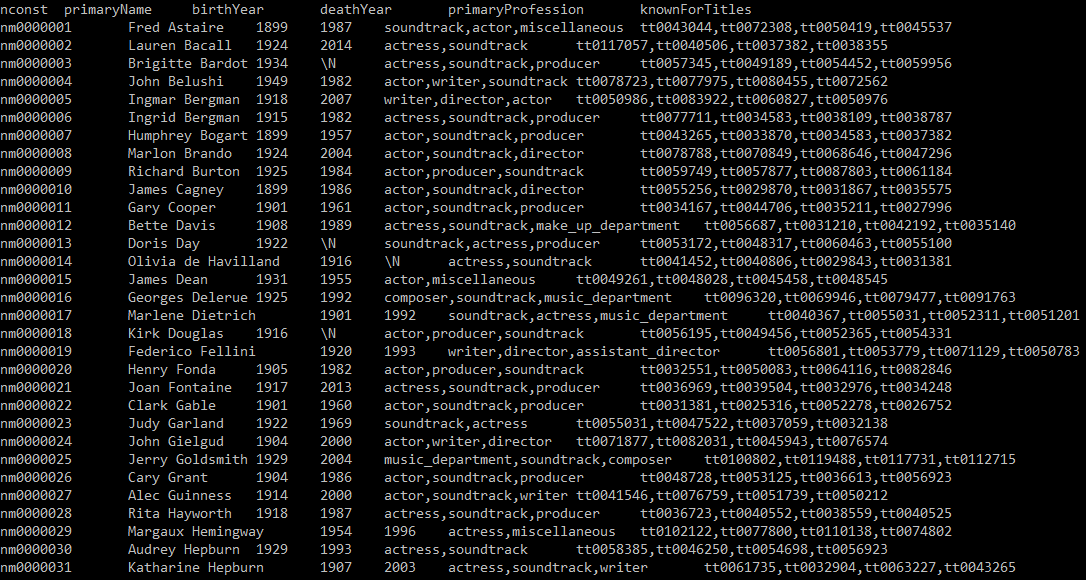
\includegraphics[width=0.8\paperwidth]{Pics/names.PNG}
			\caption{Short excerpt of the \textit{names.basics.tsv} file.}
			\label{pic:names}
		\end{figure}
	\end{frame}
	
	\subsection{Data Preprocessing}
	\begin{frame}
		\frametitle{Preprocessing the title file}
		\begin{itemize}
			\item Replace every "\textbackslash N" with "-1" \pause
			\item Excluding \pause
			\begin{itemize}
				\item \textit{originalTitle} \pause
				\item \textit{isAdult} \pause
				\item \textit{endYear} \pause
			\end{itemize}
			\item Save the rest in a dictionary with \textit{tconst} as key
		\end{itemize}
	\end{frame}

	\begin{frame}
		\frametitle{Preprocessing the names file}
		\begin{itemize}
			\item Replace every "\textbackslash N" with "-1" \pause
			\item Excluding the 2nd and 3rd profession \pause
			\item Append the the information for the first three movies \pause
			\item Append the information to the data
		\end{itemize}
	\end{frame}

	\begin{frame}
		\frametitle{Creating the database with sqlite}
		\begin{itemize}
			\item "name" (tconst) \pause
			\item "actorname" \pause
			\item "birthyear" \pause
			\item "deathyear" \pause
			\item "profession1" \pause
		    \item "movie1type" \pause
			\item "movie1primarytitle" \pause
			\item "movie1startyear" \pause
			\item "movie1runtimeminutes" \pause
			\item "movie1genre1"
		\end{itemize}
	\end{frame}

\section{Adding the Domain to PyDial}
	\subsection{Recap: Slot types}
	\begin{frame}
		\frametitle{Slot types: Informable}
		Information passed from user to system \pause		
		\begin{itemize}
			\item All slots except "name" (numerical identifier)
		\end{itemize}
	\end{frame}
	
	\begin{frame}
		\frametitle{Slot types: System Requestable}
		Information asked from user by system \pause
		\begin{itemize}
			\item Actor Name
			\item Birth Year
			\item Death Year
			\item Primary Profession
			\item International Title of each movie
			\item Premiere Year of each movie
			\item Primary Genre of each movie
		\end{itemize}
	\end{frame}
		
	\begin{frame}
		\frametitle{Slot types: Requestable}
		Information asked from system by user
		\begin{itemize}
			\item Actor Name
			\item Birth Year
			\item Death Year
			\item Primary Profession
			\item International Title of each movie
			\item Premiere Year of each movie
			\item Primary Genre of each movie
		\end{itemize}
	\end{frame}
	
	\begin{frame}
		\frametitle{Slot types: Binary}
		Boolean data\pause
		\begin{itemize}
			\item None of our slots
		\end{itemize}
	\end{frame}

\section{Limitations}
	\begin{frame}
		\frametitle{Limitations}
		\begin{figure}[ht]
			\centering
			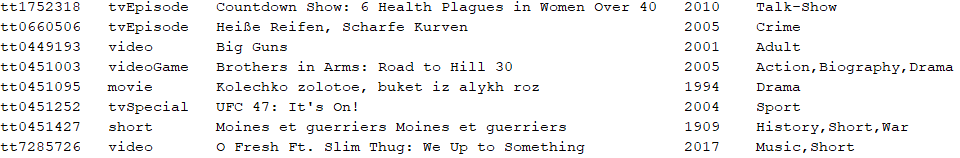
\includegraphics[width=0.9\paperwidth]{Pics/curiosities.png}
			\caption{Redundancy in the IMDB.}
			\label{pic:curiosities}
		\end{figure}
	\end{frame}	
	
	\begin{frame}
		\frametitle{Limitations: IMDB data}
		\begin{itemize}
			\item Size:\\
			Preprocessing required due to redundancy.\\ \pause
			\item Data Format:\\
			Actor names as single string\\ \pause
			"stone" robert a stone iii\\
			vs.\\
			'carl' nai peng wang\\
			vs.\\
			a. chandler warren jr.\\
		\end{itemize}
	\end{frame}
	
	\begin{frame}
		\frametitle{Limitations: PyDial}
		\begin{itemize}
			\item Hard-coded behaviour\\
			(e.g. unicode handling, "name" as primary key)\pause
			\item lacking modularity\\
			(Adding new RegEx by code instead of providing config files)\pause
			\item Creating redundant files instead of just accessing the database\pause
			\item Poor documentation
		\end{itemize}
	\end{frame}

\section{Takeaway}
\begin{frame}
	\frametitle{Remaining Tasks}
	\begin{itemize}
		\item Define remaining RegEx for keyword detection\pause
		\item Cover all possible sentence combinations for output\pause
		\item Test \& Repeat
	\end{itemize}
\end{frame}	

\begin{frame}
	\centering \Large
	\emph{\textbf{Thank you for your attention!}}
\end{frame}

\end{document}